\documentclass{article}   
\usepackage[left=1.5cm,right=1.5cm,top=2.3cm,bottom=2.3cm]{geometry}	

\usepackage[utf8]{inputenc} 										
%\usepackage[french]{babel}
\usepackage{fancyhdr}										
\usepackage{hyperref}										
\usepackage{booktabs,multirow,hhline}							
\usepackage{graphicx}									
\usepackage{wrapfig,caption}
\usepackage{subcaption}
\usepackage[compact]{titlesec}
\titlespacing{\section}{0pt}{2ex}{1ex}
\titlespacing{\subsection}{0pt}{1ex}{0ex}
\titlespacing{\subsubsection}{0pt}{0.5ex}{0ex}
\usepackage{color}												
\usepackage[dvipsnames]{xcolor}								
\usepackage{amsmath,amssymb,amsthm,nicefrac}
\usepackage{mathrsfs}										
\usepackage{wasysym,marvosym}
\usepackage{mathtools}
\usepackage{verbatim}										
\usepackage{minted}										
\usepackage{lipsum}
\usepackage{tikz}
\usepackage[american]{circuitikz}
\usepackage{siunitx}
\usepackage{physics}
\usepackage{float}
%\usepackage{biblatex}
\usepackage{movie15}
\usepackage{multicol}
%\usepackage[backend=biber, style=numeric]{biblatex}

%\newenvironment{Figure}
%{\par\medskip\noindent\minipage{\linewidth}}
  %{\endminipage\par\medskip}

\parindent=0pt									
\parskip=6pt									

\fancyheadoffset{0 cm}	

%---------------
\begin{document}
\usetikzlibrary{calc,patterns,angles,quotes}
\begin{center}

    {\Large \textbf{Quantitative assessment of spatial smoothing-induced correlations}}\\
    
    \vspace{10 pt}
    Olivier Ribordy$^{1}$ \\
    \vspace{5 pt}
    
    $^1$\textit{Département de physique, de génie physique et d'optique, Université Laval, Québec (Québec), Canada}
    

\end{center}

\vspace{10 pt}

\begin{multicols}{2}

\section*{Introduction}



\section*{Results}


\subsection*{Correlations emerging from spatial smoothing of gaussian noise signals}

We investigate the artifical introduction of correlations by the use of spatial smoothing on node activity in graphs embedded in a metric space. In the following, correlations will be taken as the Pearson correlation coefficient,  which, for a sample of variables $x$ and $y$ of size $n$, is given by
\begin{align*}
    r_{xy} = \frac{\sum_{i=1}^n(x_i-\bar{x})(y_i-\bar{y})}{\sqrt{\sum ^n _{i=1}(x_i - \bar{x})^2} \sqrt{\sum ^n _{i=1}(y_i - \bar{y})^2}},
\end{align*}
where $\bar{x}$ and $\bar{y}$ are the average values of $x$ and $y$. Since we are interested in the expected value of this coefficient for random signals, we will instead proceed with our calculations using the following coefficient:
\begin{align}
    c_{ij} &= \frac{\expval{f_if_j}-\expval{f_i}\expval{f_j}}{\sigma_{f_i}\sigma_{f_j}},
    \label{eq:exp_coefficient}
\end{align}
where $f_i$ would be the random variable corresponding to the activity of node $i$ on a observed unknown network, for instance. If we treat those signals as independent and with mean $0$, the expected coefficient is simply
\begin{align*}
    c_{ij} &= \frac{\expval{f_i}\expval{f_j}-\expval{f_i}\expval{f_j}}{\sigma_{f_i}\sigma_{f_j}} = 0.
\end{align*}
Now, we introduce spatial smoothing to the signal. This procedure consists of convoluting the signal with a gaussian filter, which yields
\begin{align*}
    \Tilde{f}_i &= \frac{1}{\sqrt{2\pi}\sigma N}\sum_{k=1}^N e^{-\nicefrac{d_{ik}^2}{2\sigma^2}}f_k,
\end{align*}
where $\sigma$ is the standard deviation of the gaussian filter, $N$ is the number of nodes in the network and $d_{ij}$ is the distance between nodes $i$ and $j$. Since all $f_k$ have mean $0$, the smoothed signals $\Tilde{f}_i$ also have mean $0$. The covariance between these smoothed signals is then
\begin{align*}
    \expval{\Tilde{f}_i\Tilde{f}_j} &= \frac{1}{2\pi\sigma^2N^2}\expval{\qty(\sum_{k=1}^N e^{-\nicefrac{d_{ik}^2}{2\sigma^2}}f_k)\qty(\sum_{\ell=1}^N e^{-\nicefrac{d_{j\ell}^2}{2\sigma^2}}f_\ell)}\\
    &= \frac{1}{2\pi\sigma^2N^2}\expval{\sum_{k, \ell =1}^N e^{\nicefrac{-(d_{ik}^2+d_{j\ell}^2)}{2\sigma^2}}f_kf_\ell}\\
    &= \frac{1}{2\pi\sigma^2N^2}\sum_{k, \ell =1}^N e^{\nicefrac{-(d_{ik}^2+d_{j\ell}^2)}{2\sigma^2}}\expval{f_kf_\ell}.
\end{align*}
Since the unsmoothed signals are independent, $\expval{f_kf_\ell} = \expval{f_k^2}\delta_{k\ell} = \sigma_{f_k}^2\delta_{k\ell}$, with $\delta_{k\ell}$ the Kronecker delta. The covariance is therefore
\begin{align*}
    \expval{\Tilde{f}_i\Tilde{f}_j} &= \frac{1}{2\pi\sigma^2N^2}\sum_{k = 1}^N e^{\nicefrac{-(d_{ik}^2+d_{jk}^2)}{2\sigma^2}}\sigma_{f_k}^2.
\end{align*}
For the standard deviations, we have
\begin{align*}
    \sigma^2_{\Tilde{f}_i} &= \expval{\Tilde{f}_i^2}\\
    &= \frac{1}{2\pi\sigma^2N^2}\expval{\qty(\sum_{k=1}^N e^{-\nicefrac{d_{ik}^2}{2\sigma^2}}f_k)\qty(\sum_{\ell=1}^N e^{-\nicefrac{d_{i\ell}^2}{2\sigma^2}}f_\ell)}\\
    &= \frac{1}{2\pi\sigma^2N^2}\expval{\sum_{k, \ell =1}^N e^{-(\nicefrac{d_{ik}^2 + d_{i\ell}^2)}{2\sigma^2}}f_kf_\ell}\\
    &= \frac{1}{2\pi\sigma^2N^2}\sum_{k=1}^N e^{-\nicefrac{d_{ik}^2}{\sigma^2}}\sigma_{f_k}^2.
\end{align*}
If all the signals are i.i.d, that is they all have the same variance, then the expected correlation between the smoothed signals is
\begin{align}
    \Tilde{c}_{ij} &= \frac{\sum_{k = 1}^N e^{\nicefrac{-(d_{ik}^2+d_{jk}^2)}{2\sigma^2}}}{\sqrt{\qty(\sum_{k=1}^N e^{-\nicefrac{d_{ik}^2}{\sigma^2}})\qty(\sum_{\ell=1}^N e^{-\nicefrac{d_{j\ell}^2}{\sigma^2}})}} \geq 0.
    \label{eq:artificial_correlation}
\end{align}
The corresponding correlation matrix is presented in figure \ref{fig:correlation matrix}.

\begin{figure}[H]
    \centering    
    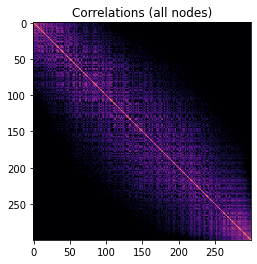
\includegraphics[width=0.3\textwidth]{figures/Theoretical correlations.png}
    \caption{Correlation matrix with entries given by equation \ref{eq:artificial_correlation}}
    \label{fig:correlation matrix}
\end{figure}

Simplifying equation \ref{eq:artificial_correlation}, as far as I can tell, requires knowledge of the metric space in which the graph is embedded, of the distribution of the nodes in that metric space and thus of the distribution of the distances between nodes. Even when this information is available, this process is arduous, but we might revisit it later for specific geometries. We can, however, try to isolate the effect of $d_{ij}$ by using the law of cosines in the exponential at the numerator, which yields
\begin{align}
    \Tilde{c}_{ij} &= e^{\nicefrac{-d_{ij}^2}{2\sigma^2}}\frac{\sum_{k = 1}^N e^{\nicefrac{-d_{ik}d_{jk}\cos(\angle ikj)}{\sigma^2}}}{\sqrt{\qty(\sum_{k=1}^N e^{-\nicefrac{d_{ik}^2}{\sigma^2}})\qty(\sum_{\ell=1}^N e^{-\nicefrac{d_{j\ell}^2}{\sigma^2}})}},
    \label{eq:gaussian_correlation}
\end{align}
with $\angle ikj$ denoting the angle between segments $ik$ and $kj$. Although this does leave a dependence on $ij$ in the numerator, equation \ref{eq:gaussian_correlation} still suggests that the smoothed correlations should decrease with distance following a curve proportional to the gaussian filter that was applied.

We can try to approximate equation \ref{eq:gaussian_correlation} to make the induced correlations more explicit. To do so, we approximate the sums in the limit of large $N$, in which case the sums should converge to an integral. This ignores the boundary effects, and as such is only valid for small $\sigma$ and nodes not too close to the boundary. For the sums at the denominator, we have

\begin{align*}
    \sum_{k=1}^N e^{-\nicefrac{d_{ik}^2}{\sigma^2}} &\approx \int_0^{2\pi}\int_0^\infty e^{-r^2/\sigma^2}r\dd r\dd\theta\\
    &= \pi\sigma^2.
\end{align*}
Since the choice of node $i$ or $j$ should have no impact on the sum, both sums at the denominator are equal, and as such the denominator as a whole is approximately $\pi\sigma^2$. 

The numerator is harder to estimate, but we can use a similar method, using the law of cosines and the following geometric construction:

\begin{center}
\begin{tikzpicture}

    % Define the center, the point on the circle, and the external point
    \coordinate (i) at (0,0); % Center of the circle
    \coordinate (k) at (1,2); % Point on the circle
    \coordinate (j) at (4,0); % Point outside the circle

    % Draw the circle
    \draw (i) circle[radius=sqrt(5)];

    % Draw the radius
    \draw[dashed] (i) -- (k);

    % Draw the lines from j to i and j to k
    \draw[dashed] (j) -- (i);
    \draw[dashed] (j) -- (k);

    % Draw the center, boundary point, and external point
    \fill (i) circle[radius=2pt];
    \fill (k) circle[radius=2pt];
    \fill (j) circle[radius=2pt];

    % Label the center, boundary point, and external point
    \node at (i) [label=left:$i$] {};
    \node at (k) [label=above:$k$] {};
    \node at (j) [label=above:$j$] {};

    % Label the radius
    \node at ($(i)!0.5!(k)$) [above left] {$r$};

    % Label the lines
    \node at ($(i)!0.4!(j)$) [below right] {$d_{ij}$};
    \node at ($(k)!0.5!(j)$) [above right] {$d_{jk}$};
    \pic [draw, ->, "$\theta$", angle eccentricity=1.5] {angle = j--i--k};
\end{tikzpicture}
\end{center}

With the law of cosines, 
\begin{equation*}
    d_{jk}^2 = r^2+d_{ij}^2-2rd_{ij}\cos\theta.
\end{equation*}
As such, the integral approximating the numerator is
\begin{align*}
    \text{num} &= \int_{0}^{2\pi}\int_0^{\infty}e^{-(r^2+r^2+d_{ij}^2-2rd_{ij}\cos\theta)/2\sigma^2}r\dd r\dd \theta\\
    &= e^{\nicefrac{-d_{ij}^2}{2\sigma^2}}\int_{0}^{2\pi}\int_0^{\infty}e^{-(r^2-rd_{ij}\cos\theta)/\sigma^2}r\dd r\dd \theta.
\end{align*}
With $a:=d_{ij}\cos\theta$, this can be written as
\begin{align*}
    \text{num} &= e^{\nicefrac{-d_{ij}^2}{2\sigma^2}}\int_{0}^{2\pi}\int_0^{\infty}e^{-(r^2-ar)/\sigma^2}r\dd r\dd \theta\\
    &= \frac{\sigma}{4} e^{\nicefrac{-d_{ij}^2}{2\sigma^2}}\int_{0}^{2\pi}\qty[\sqrt{\pi}ae^{a^2/4\sigma^2}\qty(1+\text{erf}\qty(\frac{a}{2\sigma})) + 2\sigma]\dd \theta.
\end{align*}
Now, writing $c:=\nicefrac{d_{ij}}{2\sigma}$, this is
\begin{align*}
    \text{num} &= \frac{\sigma}{4} e^{\nicefrac{-d_{ij}^2}{2\sigma^2}}\int_{0}^{2\pi}\qty[\sqrt{\pi}d_{ij}\cos\theta e^{c^2\cos^2\theta}\qty(1+\text{erf}\qty(c\cos\theta)) + 2\sigma]\dd \theta\\
    &= \frac{\sigma}{4} e^{\nicefrac{-d_{ij}^2}{2\sigma^2}}\qty[4\pi\sigma + \sqrt{\pi}d_{ij}\int_{0}^{2\pi}\cos\theta e^{c^2\cos^2\theta}\qty(1+\text{erf}\qty(c\cos\theta))\dd \theta]\\
    &= \frac{\sigma}{4} e^{\nicefrac{-d_{ij}^2}{2\sigma^2}}\qty[4\pi\sigma + \sqrt{\pi}d_{ij}\int_{0}^{2\pi}\cos\theta e^{c^2\cos^2\theta}\text{erf}\qty(c\cos\theta)\dd \theta]
\end{align*}
This last integral is the most challenging to perform. It can maybe be approximated or computed through a trigonometric substitution, but I haven't managed either yet. However, we can guarantee the following bound:

\begin{equation}
    \Tilde{c_{ij}} \geq e^{-d_{ij}^2/2\sigma^2}.
\end{equation}

One approach to approximating the integral in the equation for the numerator is to use the approximation $\text{erf}(x) \approx x$, which is roughly ok for small values of $x$. If we do so, the integrand becomes $c\cos^2\theta e^{c^2\cos^2\theta}$. This still doesn't yield a closed form for the integral as far as I can tell. 

What we can do instead is to develop the exponential and the error function into their Maclaurin series. We can then multiply the series and integrate term by term. This yields

\begin{align*}
    \text{int} &= \frac{2}{\sqrt{\pi}}\cos\theta\qty(\sum_{i=0}^\infty\frac{c^{2i}\cos^{2i}\theta}{i!})\qty(\sum_{j=0}^\infty\frac{(-1)^jc^{2j+1}\cos^{2j+1}\theta}{j!(2j+1)})\\
    &= \frac{2c}{\sqrt{\pi}}\cos^2\theta\qty(\sum_{i=0}^\infty\frac{c^{2i}\cos^{2i}\theta}{i!})\qty(\sum_{j=0}^\infty\frac{(-1)^jc^{2j}\cos^{2j}\theta}{j!(2j+1)})\\
    &= \frac{2c}{\sqrt{\pi}}\cos^2\theta\sum_{k=0}^\infty\sum_{l=0}^k\frac{(-1)^{k-l}}{l!(k-l)!(2k-2l+1)}c^{2k}\cos^{2k}\theta.
\end{align*}

\end{multicols}
\centering
\rule{0.66\textwidth}{0.4pt}

\raggedright
\vspace{10pt}
From this, we get
\begin{align*}
    \text{num} &= \frac{\sigma}{4} e^{\nicefrac{-d_{ij}^2}{2\sigma^2}}\Big[4\pi\sigma + \frac{d_{ij}^2}{\sigma}\sum_{k=0}^\infty\sum_{l=0}^k\frac{(-1)^{k-l}}{l!(k-l)!(2k-2l+1)}c^{2k}\int_{0}^{2\pi}\cos^{2k+2}\theta\dd\theta \Big]\\
    &= \frac{\sigma}{4} e^{\nicefrac{-d_{ij}^2}{2\sigma^2}}\Big[4\pi\sigma + \frac{\pi d_{ij}^2}{\sigma}\sum_{k=0}^\infty\sum_{l=0}^k\binom{2k+1}{k+1}\frac{(-1)^{k-l}}{l!(k-l)!(2k-2l+1)4^{k}}c^{2k} \Big],
\end{align*}
and finally
\begin{align}
    \Tilde{c}_{ij} &\approx e^{\nicefrac{-d_{ij}^2}{2\sigma^2}}\qty[1+\frac{d_{ij}^2}{4\sigma^2}\sum_{k=0}^\infty\qty(\sum_{l=0}^k\frac{(-1)^{k-l}}{l!(k-l)!(2k-2l+1)})\binom{2k+1}{k+1}\qty(\frac{d_{ij}^2}{16\sigma^2})^{k}].
    \label{eq:induced_correlations_series}
\end{align}
\centering
\rule{0.66\textwidth}{0.4pt}
\raggedright
\begin{multicols}{2}
One can extract as many terms as desired from eq.\ref{eq:induced_correlations_series}. As an indicator, the first few approximations would be
\begin{align}
    \Tilde{c}_{ij} &\approx e^{\nicefrac{-d_{ij}^2}{2\sigma^2}}\qty[1+\frac{d_{ij}^2}{4\sigma^2}]\\
    \Tilde{c}_{ij} &\approx e^{\nicefrac{-d_{ij}^2}{2\sigma^2}}\qty[1+\frac{d_{ij}^2}{4\sigma^2} + \frac{d_{ij}^4}{32\sigma^4}].\\
    \Tilde{c}_{ij} &\approx  e^{\nicefrac{-d_{ij}^2}{2\sigma^2}}\qty[1+\frac{d_{ij}^2}{4\sigma^2} + \frac{d_{ij}^4}{32\sigma^4} + \frac{d_{ij}^6}{384\sigma^6}].
    \label{eq:series_approximations}
\end{align}
Although I struggle to prove it, numerical tests would suggest that this series takes the simple form
\begin{align*}
    \Tilde{c}_{ij} &\approx e^{\nicefrac{-d_{ij}^2}{2\sigma^2}}\sum_{n=0}^\infty \frac{1}{n!}\qty(\frac{d_{ij}}{2\sigma})^{2n}\\
    &= e^{-\nicefrac{d_{ij}^2}{4\sigma^2}},
\end{align*}
Which is simply the filter used for the spatial smoothing, but with doubled variance and normalized. Alternatively,

\begin{align*}
    \text{num} &= \int_{0}^{2\pi}\int_0^{\infty}e^{-(r^2+r^2+d_{ij}^2-2rd_{ij}\cos\theta)/2\sigma^2}r\dd r\dd \theta\\
    &= e^{\nicefrac{-d_{ij}^2}{2\sigma^2}}\int_0^{\infty}e^{-\nicefrac{r^2}{\sigma^2}}r\dd r\int_{0}^{2\pi}e^{rd_{ij}\cos\theta/\sigma^2}\dd \theta\\
    &= 2\pi e^{\nicefrac{-d_{ij}^2}{2\sigma^2}}\int_0^{\infty}e^{-\nicefrac{r^2}{\sigma^2}}I_0\qty(\frac{d_{ij}r}{\sigma^2})r\dd r\\
    &= 2\pi e^{\nicefrac{-d_{ij}^2}{2\sigma^2}} \sum_{n=0}^\infty \frac{d_{ij}^{2m}}{(2\sigma^2)^{2m} m!^2}\int_0^\infty r^{2m+1} e^{-\nicefrac{r^2}{\sigma^2}} \dd r\\
    &= \pi \sigma^2 e^{\nicefrac{-d_{ij}^2}{2\sigma^2}} \sum_{n=0}^\infty \frac{(d_{ij}^{2})^{m}}{(4\sigma^2)^{m} m!}\\
    &= 
\end{align*}

\raggedright

\subsection*{Artifical correlations introduced to correlated systems}
We now produce a similar analysis, but for systems where the signals are not gaussian noise, and therefore $\expval{f_kf_\ell} \neq \delta_{k\ell}$. In that case,
\begin{align*}
     \expval{\Tilde{f_i}} &= \frac{1}{\sqrt{2\pi}\sigma N}\sum_{k=1}^N e^{-\nicefrac{d_{ik}^2}{2\sigma^2}}\expval{f_k}
\end{align*}
and

\begin{align*}
    \expval{\Tilde{f}_i\Tilde{f}_j} &= \frac{1}{2\pi\sigma^2N^2}\sum_{k, \ell =1}^N e^{\nicefrac{-(d_{ik}^2+d_{j\ell}^2)}{2\sigma^2}}\expval{f_kf_\ell}.
\end{align*}
For the smoothed standard deviations,
\begin{align*}
    \sigma_{\Tilde{f_i}}^2 &= \expval{\Tilde{f_i}^2} - \expval{\Tilde{f_i}}^2.
\end{align*}
Let's calculate each term separately. 
\begin{align*}
     \expval{\Tilde{f_i}}^2 &= \frac{1}{2\pi\sigma^2N^2}\sum_{k=1, \ell=1}^N e^{-\nicefrac{(d_{ik}^2+ d_{i\ell}^2)}{2\sigma^2}}\expval{f_k}\expval{f_\ell}\\
    \expval{\Tilde{f_i}^2} &= \frac{1}{2\pi\sigma^2N^2}\sum_{k=1, \ell=1}^N e^{-\nicefrac{(d_{ik}^2+ d_{i\ell}^2)}{2\sigma^2}}\expval{f_k f_\ell}\\
    \implies \sigma_{\Tilde{f_i}}^2 &= \frac{1}{2\pi\sigma^2N^2}\sum_{k=1, \ell=1}^N e^{-\nicefrac{(d_{ik}^2+ d_{i\ell}^2)}{2\sigma^2}}\qty(\expval{f_k f_\ell} - \expval{f_k}\expval{f_\ell})\\
    &= \frac{1}{2\pi\sigma^2N^2}\sum_{k=1, \ell=1}^N e^{-\nicefrac{(d_{ik}^2+ d_{i\ell}^2)}{2\sigma^2}}c_{k\ell}\sigma_{f_k}\sigma_{f_\ell}
\end{align*}
\end{multicols}
\centering
\rule{0.66\textwidth}{0.4pt}

\raggedright
\vspace{10pt}

Therefore,
\begin{align}
    \Tilde{c}_{ij} &= \frac{\sum_{k, \ell =1}^N e^{\nicefrac{-(d_{ik}^2+d_{j\ell}^2)}{2\sigma^2}}c_{k\ell}\sigma_{f_k}\sigma_{f_\ell}}{\sqrt{\qty(\sum_{k=1, \ell=1}^N e^{-\nicefrac{(d_{ik}^2+ d_{i\ell}^2)}{2\sigma^2}}c_{k\ell}\sigma_{f_k}\sigma_{f_\ell})\qty(\sum_{k=1, \ell=1}^N e^{-\nicefrac{(d_{jk}^2+ d_{j\ell}^2)}{2\sigma^2}}c_{k\ell}\sigma_{f_k}\sigma_{f_\ell})}} \nonumber \\
    &= \frac{e^{\nicefrac{-(d_{ii}^2+d_{jj}^2)}{2\sigma^2}}c_{ij}\sigma_{f_i}\sigma_{f_j} + \sum_{k\neq i, \ell \neq j}^N e^{\nicefrac{-(d_{ik}^2+d_{j\ell}^2)}{2\sigma^2}}c_{k\ell}\sigma_{f_k}\sigma_{f_\ell}}{\sqrt{\qty(\sum_{k=1, \ell=1}^N e^{-\nicefrac{(d_{ik}^2+ d_{i\ell}^2)}{2\sigma^2}}c_{k\ell}\sigma_{f_k}\sigma_{f_\ell})\qty(\sum_{k=1, \ell=1}^N e^{-\nicefrac{(d_{jk}^2+ d_{j\ell}^2)}{2\sigma^2}}c_{k\ell}\sigma_{f_k}\sigma_{f_\ell})}} \nonumber \\
    &= \frac{c_{ij}+\sum_{k\neq i, \ell \neq j}^N e^{\nicefrac{-(d_{ik}^2+d_{j\ell}^2)}{2\sigma^2}}c_{k\ell}\frac{\sigma_{f_k}\sigma_{f_\ell}}{\sigma_{f_i}\sigma_{f_j}}}{\sqrt{\qty(\sum_{k=1, \ell=1}^N e^{-\nicefrac{(d_{ik}^2+ d_{i\ell}^2)}{2\sigma^2}}c_{k\ell}\frac{\sigma_{f_k}\sigma_{f_\ell}}{\sigma_{f_i}\sigma_{f_j}})\qty(\sum_{k=1, \ell=1}^N e^{-\nicefrac{(d_{jk}^2+ d_{j\ell}^2)}{2\sigma^2}}c_{k\ell}\frac{\sigma_{f_k}\sigma_{f_\ell}}{\sigma_{f_i}\sigma_{f_j}})}}.
    \label{eq:additive_correction}
\end{align}
\begin{multicols}{2}
    The ratios of standard deviations should cancel out, or almost cancel out, given that the signals should have similar variances, or will have been centered and normalized to have variance 1. This already greatly simplifies the equation. Furthermore, as with the simpler case of an uncorrelated system, both terms at the denominator should be roughly equal if we ignore border effects. This yields the following simplification:

\begin{align*}
    \Tilde{c}_{ij} &= \frac{c_{ij}+\sum_{k\neq i, \ell \neq j}^N e^{\nicefrac{-(d_{ik}^2+d_{j\ell}^2)}{2\sigma^2}}c_{k\ell}}{\sum_{k=1, \ell=1}^N e^{-\nicefrac{(d_{ik}^2+ d_{i\ell}^2)}{2\sigma^2}}c_{k\ell}}.
\end{align*}

To make anymore progress, we need to make use of a hypothesis on the shape of the real correlations $c_{k\ell}$. It seems (\textcolor{red}{Tony j'ai besoin de sources}) that many systems exhibit exponentially spatially decreasing correlations,
\begin{equation*}
    c_{k\ell} = e^{-\gamma d_{k\ell}},
\end{equation*}
with $\gamma>0$ a tuning parameter for the rate of the decrease.

To calculate the impact, we go back to the following form for the smoothed correlations:
\begin{align*}
    \Tilde{c}_{ij} &= \frac{\sum_{k, \ell =1}^N e^{\nicefrac{-(d_{ik}^2+d_{j\ell}^2)}{2\sigma^2}}c_{k\ell}}{\sqrt{\qty(\sum_{k=1, \ell=1}^N e^{-\nicefrac{(d_{ik}^2+ d_{i\ell}^2)}{2\sigma^2}}c_{k\ell})\qty(\sum_{k=1, \ell=1}^N e^{-\nicefrac{(d_{jk}^2+ d_{j\ell}^2)}{2\sigma^2}}c_{k\ell})}}\\
    &\approx \frac{\sum_{k, \ell =1}^N e^{\nicefrac{-(d_{ik}^2+d_{j\ell}^2)}{2\sigma^2}-\gamma d_{k\ell}}}{\sum_{k=1, \ell=1}^N e^{-\nicefrac{(d_{ik}^2+ d_{i\ell}^2)}{2\sigma^2}-\gamma d_{k\ell}}}.
\end{align*}
Using the same reasoning as for the smoothed noise, these sums should be well approximated by integrals for dense enough networks and small enough $\sigma$. These integrals might be a pain to compute, but we shall try nonetheless. Let's also note that the denominator should only be a normalization factor: as such, we will focus on calculating only the numerator. We have
\end{multicols}
\centering
\rule{0.66\textwidth}{0.4pt}
\begin{align*}
    \sum_{k=1}^N\sum_{\ell=1}^N e^{-\nicefrac{(d_{ik}^2+ d_{j\ell}^2)}{2\sigma^2}-\gamma d_{k\ell}} &= \sum_{k=1}^Ne^{-\nicefrac{d_{ik}^2}{2\sigma^2}}\sum_{\ell=1}^N e^{-\nicefrac{d_{j\ell}^2}{2\sigma^2}-\gamma d_{k\ell}}\\
    &= \sum_{k=1}^Ne^{-\nicefrac{\qty(d_{ik}^2+d_{jk}^2)}{2\sigma^2}}\sum_{\ell=1}^N e^{-\nicefrac{\qty( d_{k\ell}^2-2d_{k\ell}d_{jk}\cos\angle_{jk\ell})}{2\sigma^2}-\gamma d_{k\ell}}\\
    &\approx \sum_{k=1}^Ne^{-\nicefrac{\qty(d_{ik}^2+d_{jk}^2)}{2\sigma^2}}\int_{0}^{2\pi}\int_{0}^\infty e^{-\nicefrac{\qty( r^2-2(d_{jk}\cos\theta-\sigma^2\gamma) r)}{2\sigma^2}} r \dd r \dd \theta\\
    &= \sum_{k=1}^Ne^{-\nicefrac{\qty(d_{ik}^2+d_{jk}^2)}{2\sigma^2}}\int_{0}^\infty e^{-\nicefrac{r^2}{2\sigma^2}-\gamma r} r \dd r \int_{0}^{2\pi}e^{\nicefrac{d_{jk} r \cos \theta}{\sigma^2}}\dd \theta\\
    &= 2\pi\sum_{k=1}^Ne^{-\nicefrac{\qty(d_{ik}^2+d_{jk}^2)}{2\sigma^2}}\int_{0}^\infty e^{-\nicefrac{r^2}{2\sigma^2}-\gamma r} I_0\qty(\frac{d_{jk}r}{\sigma^2})r \dd r\\,
\end{align*}
\raggedright
with $I_0(z)$ the modified Bessel function of the first kind. Expanding the Bessel function as a series, we get
\begin{align*}
    &= 2\pi\sum_{k=1}^Ne^{-\nicefrac{\qty(d_{ik}^2+d_{jk}^2)}{2\sigma^2}}\sum_{m=0}^\infty \frac{(d_{jk}^2)^m}{(4\sigma^4)^m m!^2}\int_{0}^\infty e^{-\nicefrac{r^2}{2\sigma^2}-\gamma r} r^{2m+1} \dd r\\
    &= 2\pi\sum_{k=1}^Ne^{-\nicefrac{\qty(d_{ik}^2+d_{jk}^2)}{2\sigma^2}}\sum_{m=0}^\infty \frac{(d_{jk}^2)^m}{(4\sigma^4)^m m!^2}\frac{\sigma^{2m+2} \Gamma(2m+2)}{2^{2m+2}}U\qty(m+1, \frac{1}{2}, \frac{\gamma^2\sigma^2}{4})\\
    &= \sqrt{\pi}\sum_{k=1}^Ne^{-\nicefrac{\qty(d_{ik}^2+d_{jk}^2)}{2\sigma^2}}\sum_{m=0}^\infty \frac{(d_{jk}^2)^m}{(4\sigma^2)^{m} m!} \Gamma\qty(m+\frac{3}{2}){}U\qty(m+1, \frac{1}{2}, \frac{\gamma^2\sigma^2}{4}),
\end{align*}
where $U(a, b, z)$ is Tricomi's confluent hypergeometric function. Now, inverting the order of summation, we get
\begin{align*}
    &= \sqrt{\pi}\sum_{m=0}^\infty \frac{1}{(4\sigma^2)^{m} m!} \Gamma\qty(m+\frac{3}{2}){}U\qty(m+1, \frac{1}{2}, \frac{\gamma^2\sigma^2}{4})\sum_{k=1}^N d_{jk}^{2m} e^{-\nicefrac{\qty(d_{ik}^2+d_{jk}^2)}{2\sigma^2}}\\
    &\approx \sqrt{\pi}e^{-d_{ij}^2/2\sigma^2}\sum_{m=0}^\infty \frac{1}{(4\sigma^2)^{m} m!} \Gamma\qty(m+\frac{3}{2}){}U\qty(m+1, \frac{1}{2}, \frac{\gamma^2\sigma^2}{4})\int_0^\infty r^{2m+1} e^{-r^2/\sigma^2} \dd r \int_0^{2\pi}  e^{r d_{ij}\cos{\theta}/\sigma^2}\dd\theta\\
    &= \sqrt{\pi}e^{-d_{ij}^2/2\sigma^2}\sum_{m=0}^\infty \frac{1}{(4\sigma^2)^{m} m!} \Gamma\qty(m+\frac{3}{2}){}U\qty(m+1, \frac{1}{2}, \frac{\gamma^2\sigma^2}{4})\int_0^\infty r^{2m+1} e^{-r^2/\sigma^2} I_0\qty(\frac{d_{ij}r}{\sigma^2}) \dd r \\
    &= \frac{\sqrt{\pi}}{2}\sigma^2 e^{-d_{ij}^2/2\sigma^2}\sum_{m=0}^\infty \frac{1}{4^{m}} \Gamma\qty(m+\frac{3}{2})U\qty(m+1, \frac{1}{2}, \frac{\gamma^2\sigma^2}{4})L_{-m-1}\qty(\frac{d_{ij}^2}{4\sigma^2})\\
    &= \frac{\sqrt{\pi}}{2}\sigma^2 e^{-d_{ij}^2/4\sigma^2}\sum_{m=0}^\infty \frac{1}{4^{m}} \Gamma\qty(m+\frac{3}{2})U\qty(m+1, \frac{1}{2}, \frac{\gamma^2\sigma^2}{4})L_{m}\qty(-\frac{d_{ij}^2}{4\sigma^2}),
\end{align*}
with $L_n(x)$ the Laguerre polynomials. This yields as (normalized) successive approximations (which also work as lower bounds),
\begin{align*}
    \Tilde{c}_{ij} &\approx e^{-\nicefrac{d_{ij}^2}{4\sigma^2}}\\
    \Tilde{c}_{ij} &\approx e^{-\nicefrac{d_{ij}^2}{4\sigma^2}}\qty(\frac{\gamma\sigma}{4}e^{\nicefrac{\gamma^2\sigma^2}{4}}\Gamma\qty(-\frac{1}{2}, \frac{\gamma^2\sigma^2}{4}) + \frac{1}{16}\qty(4+\sigma^2d_{ij}^2)\qty(1+\frac{\gamma^2\sigma^2}{4}+\sqrt{\pi}e^{\nicefrac{\gamma^2\sigma^2}{4}}\qty(\frac{3\gamma\sigma}{4}+\frac{\gamma^3\sigma^3}{8})\text{erfc}\qty(\frac{\gamma\sigma}{2}))).
\end{align*}
Unnormalized:
\begin{align*}
    &2\pi^2\sigma^4e^{-\nicefrac{d_{ij}^2}{2\sigma^2}}\sum_{m=0}^\infty\sum_{k=0}^\infty \frac{d_{ij}^{2k}(m+k)!}{2^{m}(2\sigma)^{2k} m!^2 k!^2}\sum_{n=0}^\infty\frac{(-\sqrt{2}\gamma\sigma)^n}{n!}\Gamma\qty(m+\frac{n}{2}+1)\\
    &= 2\pi^2\sigma^4e^{-\nicefrac{d_{ij}^2}{2\sigma^2}}\sum_{m=0}^\infty\sum_{k=0}^\infty \frac{d_{ij}^{2k}(m+k)!}{2^{m}(2\sigma)^{2k} m!^2 k!^2}\qty(m! _1F_1\qty(m+1, \frac{1}{2}; \frac{\gamma^2\sigma^2}{2})-\sqrt{2}\gamma\sigma\Gamma\qty(m+\frac{3}{2}) {}_1F_1\qty(m+\frac{3}{2}, \frac{3}{2}; \frac{\gamma^2\sigma^2}{2}))\\
    &= 2\pi^2\sigma^4e^{-\nicefrac{d_{ij}^2}{2\sigma^2}}\sum_{m=0}^\infty \frac{A_m}{2^m m!^2}\sum_{k=0}^\infty \frac{(m+k)!}{k!^2}\qty(\frac{d_{ij}^2}{4\sigma^2})^{k}\\
    &= 2\pi^2\sigma^4e^{-\nicefrac{d_{ij}^2}{2\sigma^2}}\sum_{m=0}^\infty \frac{A_m}{2^m m!}{}_1F_1\qty(m+1, 1; \frac{d_{ij}^2}{4\sigma^2})\\
    &= 2\pi^2\sigma^4e^{-\nicefrac{d_{ij}^2}{4\sigma^2}}\sum_{m=0}^\infty \frac{A_m}{2^m m!}L_m\qty(-\frac{d_{ij}^2}{4\sigma^2}),
\end{align*}
where $A_m := m! _1F_1\qty(m+1, \frac{1}{2}; \frac{\gamma^2\sigma^2}{2})-\sqrt{2}\gamma\sigma\Gamma\qty(m+\frac{3}{2}) {}_1F_1\qty(m+\frac{3}{2}, \frac{3}{2}; \frac{\gamma^2\sigma^2}{2})$, and $L_m(z)$ are the Laguerre polynomials. Now, theoretically,
\begin{align*}
    A_m = \frac{m!2^{2m+2}}{\sqrt{\pi}}\Gamma\qty(m+\frac{3}{2})H_{-2m-2}\qty(\frac{\gamma\sigma}{\sqrt{2}}),
\end{align*}
where $H_m$ are the Hermite polynomials. With $\Gamma\qty(m+\nicefrac{3}{2}) = \Gamma\qty(m+1+\nicefrac{1}{2}) = (2m+1)!! \sqrt{\pi}/2^{m+1}$, the approximation becomes
\begin{align*}
    4\pi^2\sigma^4e^{-\nicefrac{d_{ij}^2}{4\sigma^2}}\sum_{m=0}^\infty (2m+1)!!H_{-2(m+1)}\qty(\frac{\gamma\sigma}{\sqrt{2}})L_m\qty(-\frac{d_{ij}^2}{4\sigma^2}).
\end{align*}
Negative index Hermite polynomials are weird, but can be defined recursively. This yields the first few (normalized) approximations as
\begin{align*}
    \Tilde{c}_{ij}^{\text{Exp}} &\approx e^{-\nicefrac{d_{ij}^2}{4\sigma^2}}\\
    \Tilde{c}_{ij}^{\text{Exp}} &\approx e^{-\nicefrac{d_{ij}^2}{4\sigma^2}}\qty[\frac{3}{2}\qty(1-\sqrt{\frac{\pi}{2}}\gamma \sigma e^{\frac{\gamma^2\sigma^2}{2}}\text{erfc}\qty(\frac{\gamma\sigma}{\sqrt{2}})) + \frac{15}{24}\qty(\gamma^2\sigma^2+2-\sqrt{\frac{\pi}{2}}\gamma \sigma(\gamma^2\sigma^2+3) e^{\frac{\gamma^2\sigma^2}{2}}\text{erfc}\qty(\frac{\gamma\sigma}{\sqrt{2}}))\qty(\frac{d_{ij}^2}{4\sigma^2}+1)]
\end{align*}

For small $\sigma$, $A_m$ should be correctly approximated by
\begin{align*}
    A_m \approx m! _1F_1\qty(m+1, \frac{1}{2}; \frac{\gamma^2\sigma^2}{2}) = 
\end{align*}

%\begin{figure*}[t!]
%    \centering
%    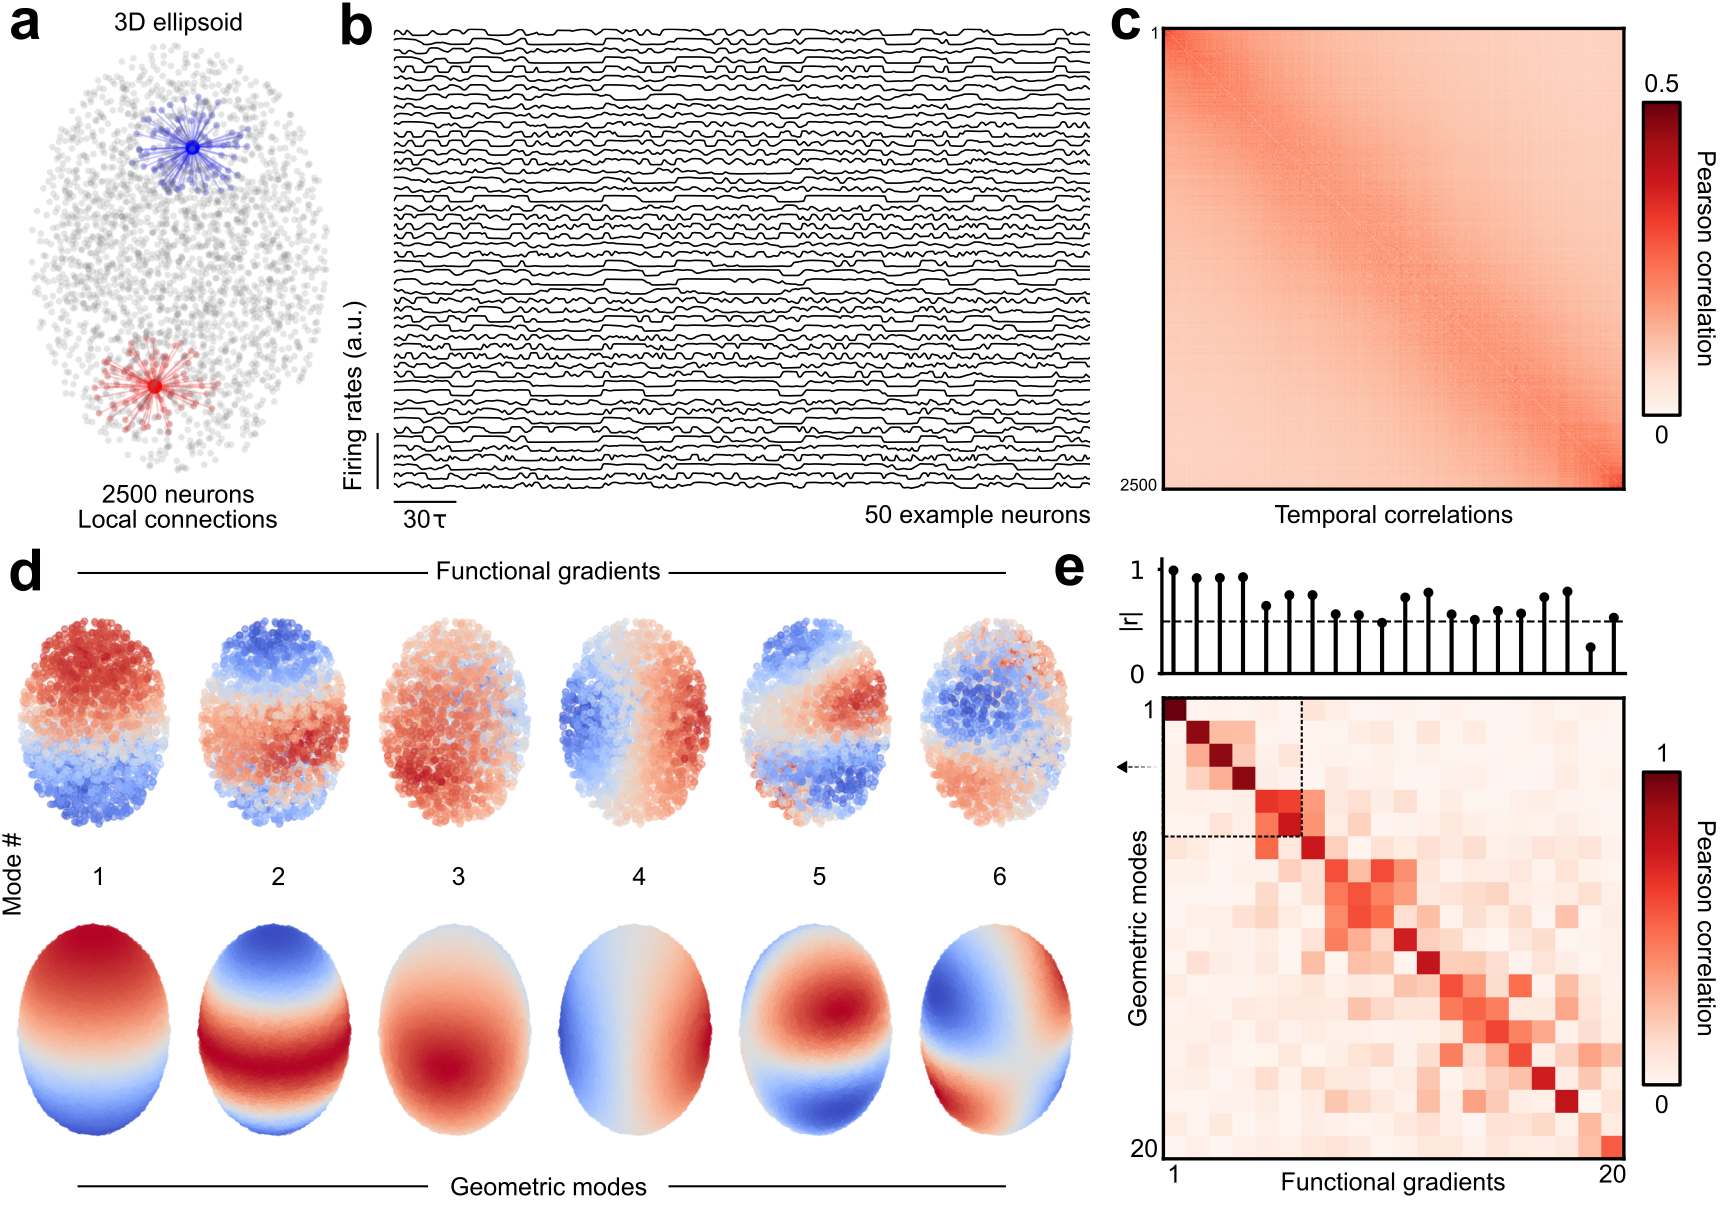
\includegraphics[width=0.95\textwidth]{Figures/figure1.png}
%    \caption{}
%    \label{fig1}
%\end{figure*}

\section*{\raggedright{Effective connection radius}}

\begin{multicols}{2}

Most of the theoretical results on the convergence of the graph laplacian to the Laplace-Beltrami operator concern random geometric graphs. In these graphs, $N$ nodes are randomly distributed (usually uniformly) in a metric space, and then connected to all nodes within a radius $h$. It is then known that as $N\to\infty$ and $h\to 0$, the graph laplacian converges to the Laplace-Beltrami operator on the metric space.

However, for other types of graphs, and notably weighted graphs, there exists no such thing as the radius of connection $h$. To study the convergence of laplacians on these graphs, we thus need an extension of that measure that captures the idea of "localness" that $h$ represents. Here, we present one such possible alternative.

For a given node $i$, take $\boldsymbol{w}_i$ to be the vector such that $w_{i, j}$ is the weight of the edge $(i, j)$, where the entries of $\boldsymbol{w}_i$ are ordered by distance from $i$, from shortest edge to longest edge. Then, we propose this measure for the effective radius of connection $h_{\text{eff}}$:

\begin{equation}
    h_{\text{eff}} := \sum_{\boldsymbol{w}_i} w_{i, j}\qty(d_{i,j}-d_{i, j-1})
\end{equation}

For a random geometric network, this simply yields $h_{\text{eff}} = h$, which was required. An advantage of this metric is that it is not sensible to border effects.

Moreover, keen eyes will recognize this as a Riemann sum. This means that in the limit $N\to\infty$, $h_{\text{eff}}$ is given by the integral
\begin{equation*}
    h_{\text{eff}} = \int_0^\infty w_{i} (x) \dd x,
\end{equation*}
where $w_{i} (x)$ is the connection strength as a function of the distance. For instance, in the correlated noise scenario,
\begin{equation*}
    w_{i} (x) = e^{-\nicefrac{x^2}{4\sigma^2}}.
\end{equation*}
This would yield $h_{\text{eff}} = \sigma\sqrt{\pi}$. In other words, the quality of mode reconstruction for smoothed gaussian noise with smoothing kernel standard deviation $\sigma$ should be equal to the quality of mode reconstruction for a random geometric graph with radius of connection $h=\sigma\sqrt{\pi}$.


\section{Connection length-preserving edge-swapping}

For a given graph, its average degree is 
\begin{align*}
    \expval{k} &= \frac{1}{N}\sum_i\sum_j a_{ij},
\end{align*}
while its average connection length is
\begin{align*}
    \expval{d} &= \frac{1}{N}\sum_i\sum_j a_{ij} d_{ij}.
\end{align*}
Each iteration of the algorithm goes as follows:
\begin{enumerate}
    \item Pick two random edges, say $(u, v)$ and $(u^\prime, v^\prime)$, at random.
    \item Say $(u^\prime, v^\prime)$ is the shortest of the two edges, $d_{u^\prime v^\prime} < d_{uv}$. Change the weight of $(u^\prime, v^\prime)$ as $a_{u^\prime v^\prime} \to a_{u^\prime v^\prime} + \min\{a_{uv}\frac{d_{uv}}{d_{u^\prime v^\prime}}, 1 - a_{u^\prime v^\prime}\}$. Conversely, change the weight of $(u, v)$ as $a_{uv} \to a_{uv} - \min\{a_{uv}, \qty(1 - a_{u^\prime v^\prime})\frac{d_{u^\prime v^\prime}}{d_{uv}}\}$.
    \item If $a_{uv}\frac{d_{uv}}{d_{u^\prime v^\prime}} < 1 - a_{u^\prime v^\prime}$, then the longer edge has been removed, and the iteration is over.
    \item If $a_{uv}\frac{d_{uv}}{d_{u^\prime v^\prime}} > 1 - a_{u^\prime v^\prime}$, then the shorter edge now has weight $1$. Choose another edge $(u^{\prime\prime}, v^{\prime\prime})$ shorter than $(u, v)$ and repeat step 2.
    \item Repeat step two a maximum of 5 times for one iteration.
\end{enumerate}
This procedure \textbf{increases} the average degree. If we instead wish to \textbf{decrease} the average degree, the same procedure can be used by choosing $(u^\prime, v^\prime)$ to be the \textbf{longer} edge instead.
\end{multicols}

\end{document}